\subsection{\bf RQ3. Overlapping Analysis}



{\footnotesize{
\definecolor{mygray}{gray}{.9}
\begin{table}[t]
	\caption{RQ3. Overlapping Analysis. The number in the gray boxes: the unique bugs that the current approach can fix. P: The percentage of the bugs that are unique ones.}
	\begin{center}
		\renewcommand{\arraystretch}{1}
		\begin{tabular}{p{0.8cm}<{\centering}|p{1.1cm}<{\centering}|p{0.8cm}<{\centering}|p{0.7cm}<{\centering}|p{1.1cm}<{\centering}|p{0.8cm}<{\centering}|p{0.7cm}<{\centering}}\hline
			Dataset&\multicolumn{3}{c|}{Bugs.jar (1,158 Bugs)}&\multicolumn{3}{c}{BigFix (2,176 Bugs)}\\
			\hline
			             & CODIT   & Overlap   & \tool  & CODIT   & Overlap   & \tool \\
			\hline
			Fixed \#     & \cellcolor{mygray} 6  & 80   & \cellcolor{mygray} 91  & \cellcolor{mygray} 13 &  157  & \cellcolor{mygray} 165 \\
			P            & 6.8\%   &    & 53.4\%  & 7.7\%   &    & 51.4\% \\
			\hline
			             & Tufano 19'   & Overlap   & \tool  & Tufano 19'   & Overlap   & \tool \\
			\hline
			Fixed \#     & \cellcolor{mygray} 5  &  71  & \cellcolor{mygray} 101 & \cellcolor{mygray}4 & 85   & \cellcolor{mygray}237 \\
			P            &  6.2\%  &    &  58.8\% &  4.9\%  &    & 73.6\% \\
			\hline
			             & SequenceR   & Overlap   & \tool  & SequenceR   & Overlap   & \tool \\
			\hline
			Fixed \#     & \cellcolor{mygray} 7  &   95 & \cellcolor{mygray} 76 & \cellcolor{mygray} 23 &  158  & \cellcolor{mygray} 164 \\
			P            &   6.8\% &    & 44.6\%  &   11.2\% &    & 50.9\% \\
			\hline
			             & DLFix   & Overlap   & \tool  & DLFix   & Overlap   & \tool \\
			\hline
			Fixed \#     & \cellcolor{mygray}  19 &  105  & \cellcolor{mygray} 66 & \cellcolor{mygray}35 &  211  & \cellcolor{mygray}111 \\
			P            &  15.0\%  &    & 38.5\%  &  14.2\%  &    &  34.5\%\\
			\hline
			             & CoCoNut   & Overlap   & \tool  & CoCoNut   & Overlap   & \tool \\
			\hline
			Fixed \#     & \cellcolor{mygray} 20  & 120   & \cellcolor{mygray} 51 & \cellcolor{mygray}44 &  226  & \cellcolor{mygray} 96\\
			P            &  14.0\%  &    &  29.7\% &  16.1\%  &    & 29.7\% \\
			\hline
			             & CURE   & Overlap   & \tool  & CURE   & Overlap   & \tool \\
			\hline
			Fixed \#     & \cellcolor{mygray} 27  &  126  & \cellcolor{mygray} 45 & \cellcolor{mygray} 50&  233  & \cellcolor{mygray} 89\\
			P            &  17.4\%  &    & 26.4\%  & 17.7\%   &    &  27.7\%\\
			\hline
		\end{tabular}
		\label{RQ3_results}
	\end{center}
\end{table}
}}


Table~\ref{RQ3_results} shows the overlapping analysis of the bugs fixed by {\tool} and the studied baselines. The results show that {\tool} can fix more unique bugs than any compared baseline. For example, {\tool} can fix 89 bugs that cannot be fixed by CURE, while CURE can fix 50 bugs that our {\tool} cannot fix. %{\tool} can fix more bugs than the studied baselines and also complement with each other
Consolidating results from RQ2 and RQ3, overall, {\tool} can auto-fix more bugs and unique bugs than any studied baselines, indicating that {\tool} is better and complementary to other baselines.


\begin{figure}[t]
	\centering
	\lstset{
		numbers=left,
		numberstyle= \tiny,
		keywordstyle= \color{blue!70},
		commentstyle= \color{red!50!green!50!blue!50},
		frame=shadowbox,
		rulesepcolor= \color{red!20!green!20!blue!20} ,
		xleftmargin=1.5em,xrightmargin=0em, aboveskip=1em,
		framexleftmargin=1.5em,
		numbersep= 5pt,
		language=Java,
		basicstyle=\scriptsize\ttfamily,
		numberstyle=\scriptsize\ttfamily,
		emphstyle=\bfseries,
		moredelim=**[is][\color{red}]{@}{@},
		escapeinside= {(*@}{@*)}
	}
	\begin{lstlisting}[]
public void visit(LOProject project) throws VisitorException {
    ...
(*@{\color{red}{-	\quad else if( op instanceof LOProject ) \{ }}@*)
(*@{\color{cyan}{+ \quad	else if( op instanceof ExpressionOperator ) \{}}@*)
		LogicalExpression expOper = exprOpsMap.get(op);
	...
	if (currentOp instanceof ExpressionOperator) {
		LogicalExpression exp = exprOpsMap.get(currentOp);
	...
}
	\end{lstlisting}
	\caption{The Example for Comparing with CODIT}
	\label{example_1}
\end{figure}


{\color{blue}{1. CODIT only do the prediction and token generation on the buggy sub-tree that covers all edited nodes without considering the other information in the same method. So it cannot catch the information about the variable $ExpressionOperator$ in the method.
2. Fixing results: \textit{CODIT: else if( op )$ \{$}
CDFIX: \textit{else if( op instanceof ExpressionOperator ) $\{$}}}

\begin{figure}[t]
	\centering
	\lstset{
		numbers=left,
		numberstyle= \tiny,
		keywordstyle= \color{blue!70},
		commentstyle= \color{red!50!green!50!blue!50},
		frame=shadowbox,
		rulesepcolor= \color{red!20!green!20!blue!20} ,
		xleftmargin=1.5em,xrightmargin=0em, aboveskip=1em,
		framexleftmargin=1.5em,
		numbersep= 5pt,
		language=Java,
		basicstyle=\scriptsize\ttfamily,
		numberstyle=\scriptsize\ttfamily,
		emphstyle=\bfseries,
		moredelim=**[is][\color{red}]{@}{@},
		escapeinside= {(*@}{@*)}
	}
	\begin{lstlisting}[]
private Tuple readFromMemory() {
    if (mContents.size() == 0) return null;
    if (mMemoryPtr < mContents.size()) {
(*@{\color{red}{-\quad\quad\quad     return ((ArrayList<Tuple>)mContents).get(mMemoryPtr++);}}@*)
(*@{\color{cyan}{+\quad\quad\quad    return ((List<Tuple>)mContents).get(mMemoryPtr++);}}@*)
	} else {
        return null;
	}
}
	\end{lstlisting}
	\caption{The Example for Comparing with Tufano 19'}
	\label{example_2}
\end{figure}


{\color{blue}{1. Tufano 19' learns and makes prediction only on the method level. In this case, it may fix the wrong position.
2. Fixing results: 
Tufano 19': \textit{if (mMemoryPtr.size() == 0) return null;} (this fix at line 2)
CDFIX: \textit{return ((List<Tuple>)mContents).get(mMemoryPtr++);}}}

\begin{figure}[t]
	\centering
	\lstset{
		numbers=left,
		numberstyle= \tiny,
		keywordstyle= \color{blue!70},
		commentstyle= \color{red!50!green!50!blue!50},
		frame=shadowbox,
		rulesepcolor= \color{red!20!green!20!blue!20} ,
		xleftmargin=1.5em,xrightmargin=0em, aboveskip=1em,
		framexleftmargin=1.5em,
		numbersep= 5pt,
		language=Java,
		basicstyle=\scriptsize\ttfamily,
		numberstyle=\scriptsize\ttfamily,
		emphstyle=\bfseries,
		moredelim=**[is][\color{red}]{@}{@},
		escapeinside= {(*@}{@*)}
	}
	\begin{lstlisting}[]
public int getPartition(PigNullableWritable wrappedKey, Writable value, int numPartitions) {
	....
	indexes = reducerMap.get(keyTuple);
	// if the reducerMap does not contain the key, do the default hash based partitioning
	if (indexes == null) {
(*@{\color{red}{-\quad\quad\quad  return (Math.abs(keyTuple.hashCode()) \% totalReducers);	}}@*)
(*@{\color{cyan}{+\quad\quad\quad     return (Math.abs(keyTuple.hashCode() \% totalReducers));}}@*)
	}
	....
}
	\end{lstlisting}
	\caption{The Example for Comparing with SequenceR, CoCoNut, DLFix, and CURE}
	\label{example_3}
\end{figure}

\begin{figure}[t]
	\centering
	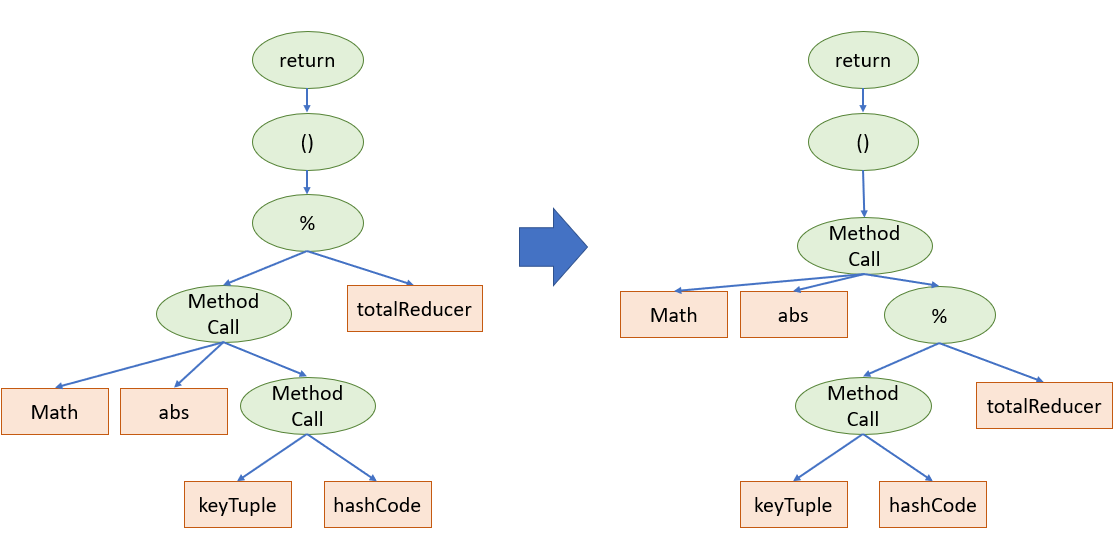
\includegraphics[width=3.2in]{graphs/example_3.png}
	\caption{AST Structure Changes in Example 3}
	\label{example_3_tree}
\end{figure}

{\color{blue}{1. SequenceR, CoCoNut, CURE all using sequence structure to do the code fixing. However, it is hard for them to learn the structure changes in this example. DLFix learns the structure changes, but it does not learn it as well as CDFix.
2. Fixing results: 
SequenceR: \textit{return (Math.abs( keyTuple.get()) \% totalReducers);}
CoCoNut: \textit{return (Math.abs( keyTuple.hashCode()));}
DLFix: \textit{return (Math.abs( keyTuple.hashCode()) \% curIndex);}
CURE: \textit{return (Math.abs( keyTuple.hashCode()) / totalReducers);}
CDFIX: \textit{return (Math.abs( keyTuple.hashCode() \% totalReducers));}}}
